\documentclass{beamer}
\usetheme{metropolis}           % Use metropolis theme
\usepackage[german]{babel}  
\usepackage[utf8]{inputenc}	%dt Sonderzeichen wie ß
\usepackage{tikz}
\usepackage{amssymb}
\usepackage{multirow}
\usepackage{pgfpages}
\usepackage{cite}
\usepackage{graphicx}
\usepackage{animate}

\usepackage{multimedia}

%\setbeameroption{show notes on second screen=right}  %% Uncomment this to get Notes


\renewcommand*{\figurename}{Abb.}




\title{Efficient and Robust Automated Machine Learning}
\date{12. Juli 2018}
\author{Robert Feldhans}
\institute{Seminar Musterklassifikation}
\begin{document}
	\maketitle
	
	\begin{frame}{Inhalt}
		\setbeamertemplate{section in toc}[sections numbered]
		\tableofcontents[hideallsubsections]
	\end{frame}
	
	\section{Motivation}%%%%%%%%%%%%%%%%%%%%%%%%%%%%%%%%%%%%%%%%%%%%%%%%%%%%%%%%%%%%%%%%%%%%%
	
	\begin{frame}{Interlude: Hyperparameter I}
		Was sind Hyperparameter?
		\begin{itemize}
			\item Werden \emph{vor} dem Lernen definiert
			\item Sind in der Regel Zahlen oder Funktionen
		\end{itemize}
		\pause
		\begin{alertblock}{Allgemein}
			Alles was in irgendeiner Art austauschbar ist in einem speziellen ML-Verfahren und während des Trainings konstant bleibt
		\end{alertblock}
	\end{frame}
	
	\begin{frame}{Interlude: Hyperparameter II}
		Beispiele für Hyperparameter
		\begin{itemize}
			\item Lernrate
			\item Gewichte jeglicher Form
			\item Anzahl der Cluster in k-means clustering
			\item Aktivierungsfunktionen
			\item Anzahl der Hidden Layers in einem Netz
			\item Breite der Layers in einem Netz
		\end{itemize}
	\end{frame}
	
	\begin{frame}{Motivation}
		\begin{itemize}
			\item Ein gutes neuronales Netz zu trainieren ist schwer, braucht viel Arbeitszeit und Erfahrung
			\item Jeder sollte in der Lage sein NN zu trainieren (im besten Fall sogar Maschinen!)
		\end{itemize}
		\pause
		\alert{Lösung: Ein automatisches (und effizientes) System, welches gute Hyperparameter auswählt, muss her!}
	\end{frame}
	
	
	\section{Automated Machine Learning in a Nutshell}%%%%%%%%%%%%%%%%%%%%%%%%%%%%%%%%%%%%%%%%%%%%%%%%%%%%%%%%%%%%%%%%%%%%%%%%%%%%%%%%
	
	
	\begin{frame}{Auto-ML I}
		\begin{alertblock}{Grundlegende Idee}
			\begin{itemize}
				\item Starten mit \emph{irgendwie} ausgewählten Hyperparametern
				\item Classifier trainieren
				\item Classifier evaluieren
				\item Hyperparametertuning mithilfe eines Bayesian optimizer
				\item Wiederholung bis zu einem zufriedenstellenden Ergebnis
			\end{itemize}
		\end{alertblock}
	\end{frame}
	
	\begin{frame}{Auto-ML II}
		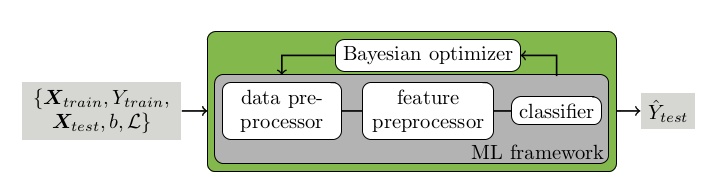
\includegraphics[width=\linewidth]{Bilder/MachineLeaningInANutshell}
	\end{frame}
	
	\begin{frame}{Initialisierung der Hyperparameter}
		Bild zu problemen mit der initialisierung von hyperparametern
	\end{frame}
	
	\begin{frame}{Rapidly Exploring Random Tree (RTT) I}
		\begin{alertblock}{Idee}
			\begin{itemize}
				\item Werte zufällig wählen
				\item So oft wiederholen, bis man einen guten Überblick über den Searchspace hat
			\end{itemize}
		\end{alertblock}
		\pause
		\begin{alertblock}{Vorteil}
			Bietet beliebig guten Überblick über den Searchspace
		\end{alertblock}
		\pause
		\begin{alertblock}{Achtung}
			RTT bietet einige Fallstricke. Think before use!
		\end{alertblock}
	\end{frame}
	
	\begin{frame}{Rapidly Exploring Random Tree (RTT) II}
		\centering
		\movie[width=1.0\textwidth,poster,autostart,showcontrols,loop]{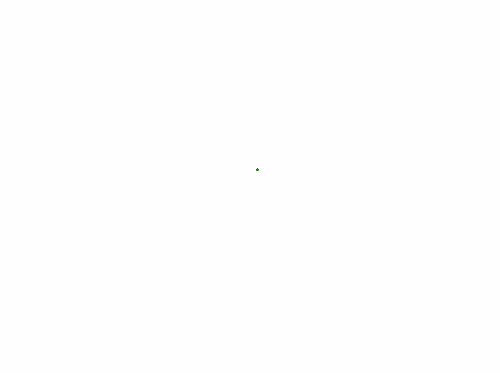
\includegraphics[width=1.0\textwidth]{Bilder/RTT-0.png}}{Bilder/RTT.mp4}
	\end{frame}
	
	\begin{frame}{Probleme}
		\begin{itemize}
			\item Ausgesprochen Rechenintensiv
			\item Unterschiedliche Lernverfahren?
			\item Es gibt kein ``best'' Lernverfahren, nur ``best at''
			\item Manche ML-Verfahren erfordern intensive Hyperparameteroptimisierung
			\item Bayes optimization sollte sich jedoch um dieses Problem kümmern
		\end{itemize}
	\end{frame}
	
	\section{Meta Learning}%%%%%%%%%%%%%%%%%%%%%%%%%%%%%%%%%%%%%%%%%%%%%%%%%%%%%%%%%%%%%%%%%%%%%%%%%%%%%%%%
	
	\begin{frame}{Meta Learning}
		\begin{alertblock}{Idee}
			\begin{itemize}
				\item Das richte ML-Verfahren für ein bestimmtes Datenset hängt vom Datenset selbst ab
				\item Ein bestimmter Klassifikator sollte auf ähnlichen Datensets ähnlich gute Ergebnisse liefern
				\pause
			\end{itemize}
			$\Rightarrow$ Also bauen wir uns einen Klassifikator, der uns anhand eines neuen Datensets sagt, welche Art von Klassifikator wir trainieren sollten
		\end{alertblock}
	\end{frame}
	
	\begin{frame}{Im Detail}
		\begin{alertblock}{Erstellung des Meta-Klassifikators}
			\begin{itemize}
				\item Für eine (große) Menge an bereits bekannten Sets: Metafeatures berechnen \\ $\Rightarrow$ class-probability, categorical-numerical-ratio, number of classes/features/instances (missing)
				\item Einen Klassifikator (SMAC) auf diesen Meta-Features trainieren
			\end{itemize}
		\end{alertblock}
		\pause
		\begin{alertblock}{Auswertung}
			\begin{itemize}
				\item Für ein neues Datenset werden anhand der $L_1$ Distanz zu den bereits bekannten Datensets Klassifikatoren ausgewählt
			\end{itemize}
		\end{alertblock}
	\end{frame}
	
	% FORMICA
	% flexible, framework
	% observatory, of
	% robust, robotic 
	% modular
	% interdisziplanary
	% cognitive
	% ants
	
	\section{Ensembles}%%%%%%%%%%%%%%%%%%%%%%%%%%%%%%%%%%%%%%%%%%%%%%%%%%%%%%%%%%%%%%%%%%%%%%%%%%%%%%%%
	
	\begin{frame}{Bestandsaufnahme}
		\begin{itemize}
			\item Mehrere vielversprechende ML-Verfahren ausgewählt
			\item Jedes davon aufwändig mit Bayesian optimizer im Hinblick auf Hyperparameter getunt
			\item Das beste der Besten herausgepickt und die anderen weggeworfen
		\end{itemize}
		\pause
		\alert{\LARGE{Warum eigentlich?}}
	\end{frame}
	
	\begin{frame}{Ensembles}
		\begin{alertblock}{Idee}
			\begin{itemize}
				\item Anstatt teuer optimierte Klassifikatoren wegzuwerfen, Kombination der Besten
			\end{itemize}
		\end{alertblock}
		\pause
		\alert{Aber wie kombinieren?}
		\begin{itemize}
			\item Alle ungewichtet aufsummieren?
			\item Stacking?
			\item gradient-free numerical optimization?
		\end{itemize}
	\end{frame}
	
	\begin{frame}{Ensemble Selection}
		\begin{alertblock}{Wie baut man ein Ensemble?}
			\begin{itemize}
				\item Starte mit einem leeren Ensemble
				\item Füge den Klassifikator dem Ensemble hinzu, der das Ensemble am besten ergänzt
				\item Wiederhole bis alle Klassifikatoren enthalten sind oder X mal
				\item Durchschnitt über alle Predictions bilden für Resultat
				\pause
				\item Alle Einträge sind ungewichtet
				\item Duplikationen sind erlaubt
			\end{itemize}
	\end{alertblock}
	\end{frame}
	
	
	\section{Anwendung und Ergebnisse}%%%%%%%%%%%%%%%%%%%%%%%%%%%%%%%%%%%%%%%
	
	\begin{frame}{Anwendung und Evaluation}
		\begin{alertblock}{Setup}
			\begin{itemize}
				\item Meta-learning mit 38 Features für 24h auf 140 OpenML Datensets (2/3 zu 1/3)
				\item Bayesian optimizer auf den 25 besten, Ensemble mit Größe 50
			\end{itemize}
		\end{alertblock}
		\pause
		\begin{alertblock}{Auffälligkeiten und Ergebnisse}
			\begin{itemize}
				\item Meta-learning und Ensemble Selection verbessert bisherige Ansätze deutlich
				\item Besonders bei kurzer Rechenzeit performt die Kombination ML+ES signifikant besser
				\item Mithilfe von ML+ES wird in der Regel ein hinreichend optimaler Klassifikator gefunden
			\end{itemize}
		\end{alertblock}
	\end{frame}
	
	\begin{frame}{Hinreichende Optimalität}
		\begin{figure}[ht]
			\centering
			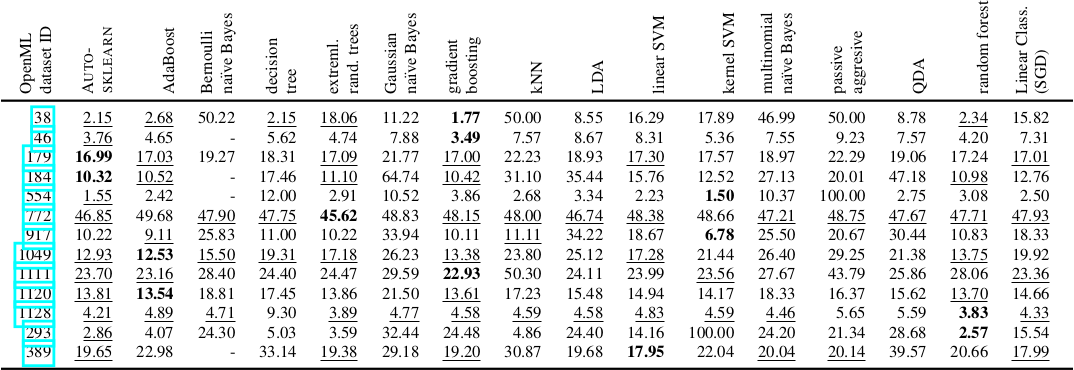
\includegraphics[width=\linewidth]{Bilder/HinreichendeOptimalitaet}
			\caption{Median balanced test error rate (BER) of optimizing AUTO - SKLEARN subspaces for each classification SVM method}
		\end{figure}
	\end{frame}
	
	\begin{frame}{Recap}
		\begin{alertblock}{Errungenschaften}
			\begin{itemize}
				\item Automatisiertes Maschinenlernen!
				\item Gute Ergebnisse sind auch ohne Vorwissen oder genaue Kenntnisse der einzelnen Verfahre möglich
			\end{itemize}
		\end{alertblock}
		\pause
		\begin{alertblock}{bleibende/ ungelöste Probleme}
			\begin{itemize}
				\item Rechenkosten
				\item Für sehr rechenaufwendige Verfahren (z.b. Deep Learning) nur eingeschränkt zu gebrauchen
				\pause
				\item Wird aber durch recht gute Parallelisierbarkeit teilweise wieder ausgeglichen 
			\end{itemize}
		\end{alertblock}
	\end{frame}
	
	
	\begin{frame}{}
			Vielen Dank für eure Aufmerksamkeit!
	\end{frame}
	
	\section{Fragerunde}%%%%%%%%%%%%%%%%%%%%%%%%%%%%%%%%%%%%%%%%%%%%%%%%%%%%%%%%%%%%%%%%%%%%%%%%%%%%%%%%%%%%%%%%%
	
	\begin{frame}{Quellen}
		\bibliography{demo}
		\bibliographystyle{plain}
	\end{frame}
	
\end{document}
	
	
	